\section{Metodologia de Trabalho}
Nesta seção serão expostos os procedimentos relativos à metodologia de trabalho da equipe de desenvolvimento.

\subsection{Ferramentas de planejamento}
O planejamento das atividades da equipe de desenvolvimento será baseado em tarefas (\glspl{issue}), que  serão criadas na área de gestão de projeto do repositório ``\textbf{participacao-sitebase}''\footnote{\textbf{participacao-sitebase} é o repositório principal do projeto e está hospedado no endereço: \url{https://github.com/pensandoodireito/participacao-sitebase/issues} - Acessado em 02/04/2015}. Cada \gls{issue} deve ser minimalista, ou seja, deve-se buscar a criação de tarefas que sejam as mais simples possíveis.

A visualização e organização dessas tarefas se dará por meio da ferramenta chamada HuBoard%
\footnote{HuBoard - \url{https://huboard.com} - Acessado em 02/04/2015}%
, que é uma interface no estilo KanBan%
\footnote{O ``sistema KanBan'' é a materialização do sistema \textit{just-in-time} e foi desenvolvido por Taiichi Ohno, enquanto Vice-Presidente da Toyota Motors na década de 1950. Ele é um sistema de controle de fluxo de atividades que se utiliza de cartões. - \url{http://en.wikipedia.org/wiki/Kanban} - Acessado em: 02/04/2015}
\cite{sugimori1977toyota},
para gerenciamento de \glspl{issue} de repositórios no GitHub%
\footnote{GitHub - repositório de projetos - \url{http://github.com} - Acessado em 02/04/2015}.

No \textit{HuBoard} tem-se 4 estados para as tarefas:
\begin{description}
\item[Backlog] - tarefas criadas e ainda não alocadas;
\item[Pronto para Trabalhar] - tarefas que devem ser trabalhadas no presente ciclo;
\item[Trabalhando] - tarefas que estão sendo desenvolvidas no momento; e
\item[Feito] - tarefas que já foram finalizadas mas ainda não avaliadas pela equipe.
\end{description}

Além do \textit{GitHub} e do \textit{HuBoard}, a equipe também utilizará o serviço chamado \textit{slack}\footnote{Slack - \url{http://slack.com} - Acessado em 04/04/2015} como ferramenta de comunicação interna. Para melhorar a comunicação o \textit{HuBoard} também será integrado ao \textit{slack}, de maneira que qualquer mudança ocorrida no \textit{HuBoard} seja registrada no \textit{slack}.

\subsection{Rotina de Planejamento e Acompanhamento}
O primeiro pressuposto da presente metodologia é que serão estabelecidos ciclos de desenvolvimento de uma semana. Para tanto, foi definido que às segundas-feiras serão realizadas as reuniões semanais de alinhamento e planejamento.

Nesta reunião, a primeira tarefa a ser realizada é a avaliação das atividades desenvolvidas desde a reunião de planejamento anterior.
Essa avaliação se dá inicialmente pela verificação de cada uma das \glspl{issue} presentes no estado \textbf{Feito} do \textit{HuBoard}. Para verificar a implementação de uma \gls{issue}, a equipe acompanhará a pessoa no papel de \textbf{integrador} implementando o \gls{pullrequest} relativo àquela \gls{issue}, validando o resultado final e em seguida arquivando a mesma.

Após a verificação de todas as \glspl{issue} no estado \textbf{Feito}, a equipe verificará se alguma \gls{issue} prevista para aquele \gls{sprint} não foi implementada. Esta checagem ocorrerá por meio da verificação da \gls{milestone}, utilizando os filtros do HuBoard. Caso todas as \glspl{issue} tenham sido implementadas, o \gls{milestone} pode ser encerrado, caso contrário, deve-se avaliar o motivo de não se ter atingido o objetivo planejado e as \glspl{issue} não implementadas voltam para a etapa de planejamento.

A seguir procede-se para a etapa de planejamento, que compreende a criação de novas \glspl{issue} em decorrência do trabalho que fora desenvolvido e também de demandas ``externas'' e de ``clientes''. Após a criação e avaliação de todas as \glspl{issue}, a equipe deve decidir quais serão trabalhadas no próximo \gls{sprint} semanal, alocando-as ao \gls{milestone} respectivo.  

Por fim, espera-se que a equipe faça um rápido acompanhamento diário das atividades junto ao gestor da equipe. Este acompanhamento tem a finalidade maior de identificar alguma atividade que está consumindo um tempo excessivo e, eventualmente, reduzir sua prioridade em detrimento de outras tarefas a serem realizadas durante o \gls{sprint}.
%TODO FAZER UM DIAGRAMA DESSE PROCESSO DE GESTÃO

\subsection{Processo e fluxo de desenvolvimento}
Para o processo e fluxo de desenvolvimento resume-se aqui, na Figura \ref{fig:gitflow} o proposto em \citeonline{rabatone2015}.

Do diagrama, destacam-se as seguintes regras:
\begin{enumerate}
\item Os desenvolvedores trabalharão em seus próprios \glspl{fork};
\item todo desenvolvimento deve ocorrer em \glspl{branch} criada para cada \gls{issue};
\item a criação de uma nova \gls{branch} deve ser realizada a partir da \gls{branch} \textbf{master}.
\begin{lstlisting}[language=bash,caption={Sugestão de comando para criar nova branch baseada na master}]
git checkout -b issueXX master
\end{lstlisting}
\item ao encerrar o desenvolvimento em uma \gls{branch} o desenvolvedor deve fazer um \gls{pullrequest} para a \gls{branch} \textbf{master} do repositório principal.
\item os desenvolvedores devem sempre manter sua \gls{branch} \textbf{master} local sincronizada com a \gls{branch} \textbf{master} do repositório principal.
\end{enumerate}

Além disso, quando for necessário realizar algum desenvolvimento emergencial para resolver problemas no sistema que está em produção, será utilizado o expediente de \gls{hotfix}. Para tanto, o desenvolvedor responsável por implementar a solução deverá criar uma nova \gls{branch} baseada na \gls{branch} \textbf{production} do repositório principal, desenvolver a solução nesta \gls{branch} e, em seguida, realizar um \gls{pullrequest} para a \gls{branch} \textbf{production} do repositório principal e outro \gls{pullrequest} para a \gls{branch} \textbf{master} do repositório principal. Em seguida o responsável pelo projeto deve ser informado para que possa ocorrar a integração dos \glspl{pullrequest} e o \gls{deploy} no site em produção.

    \begin{figure}[htb]%
        \begin{center}
            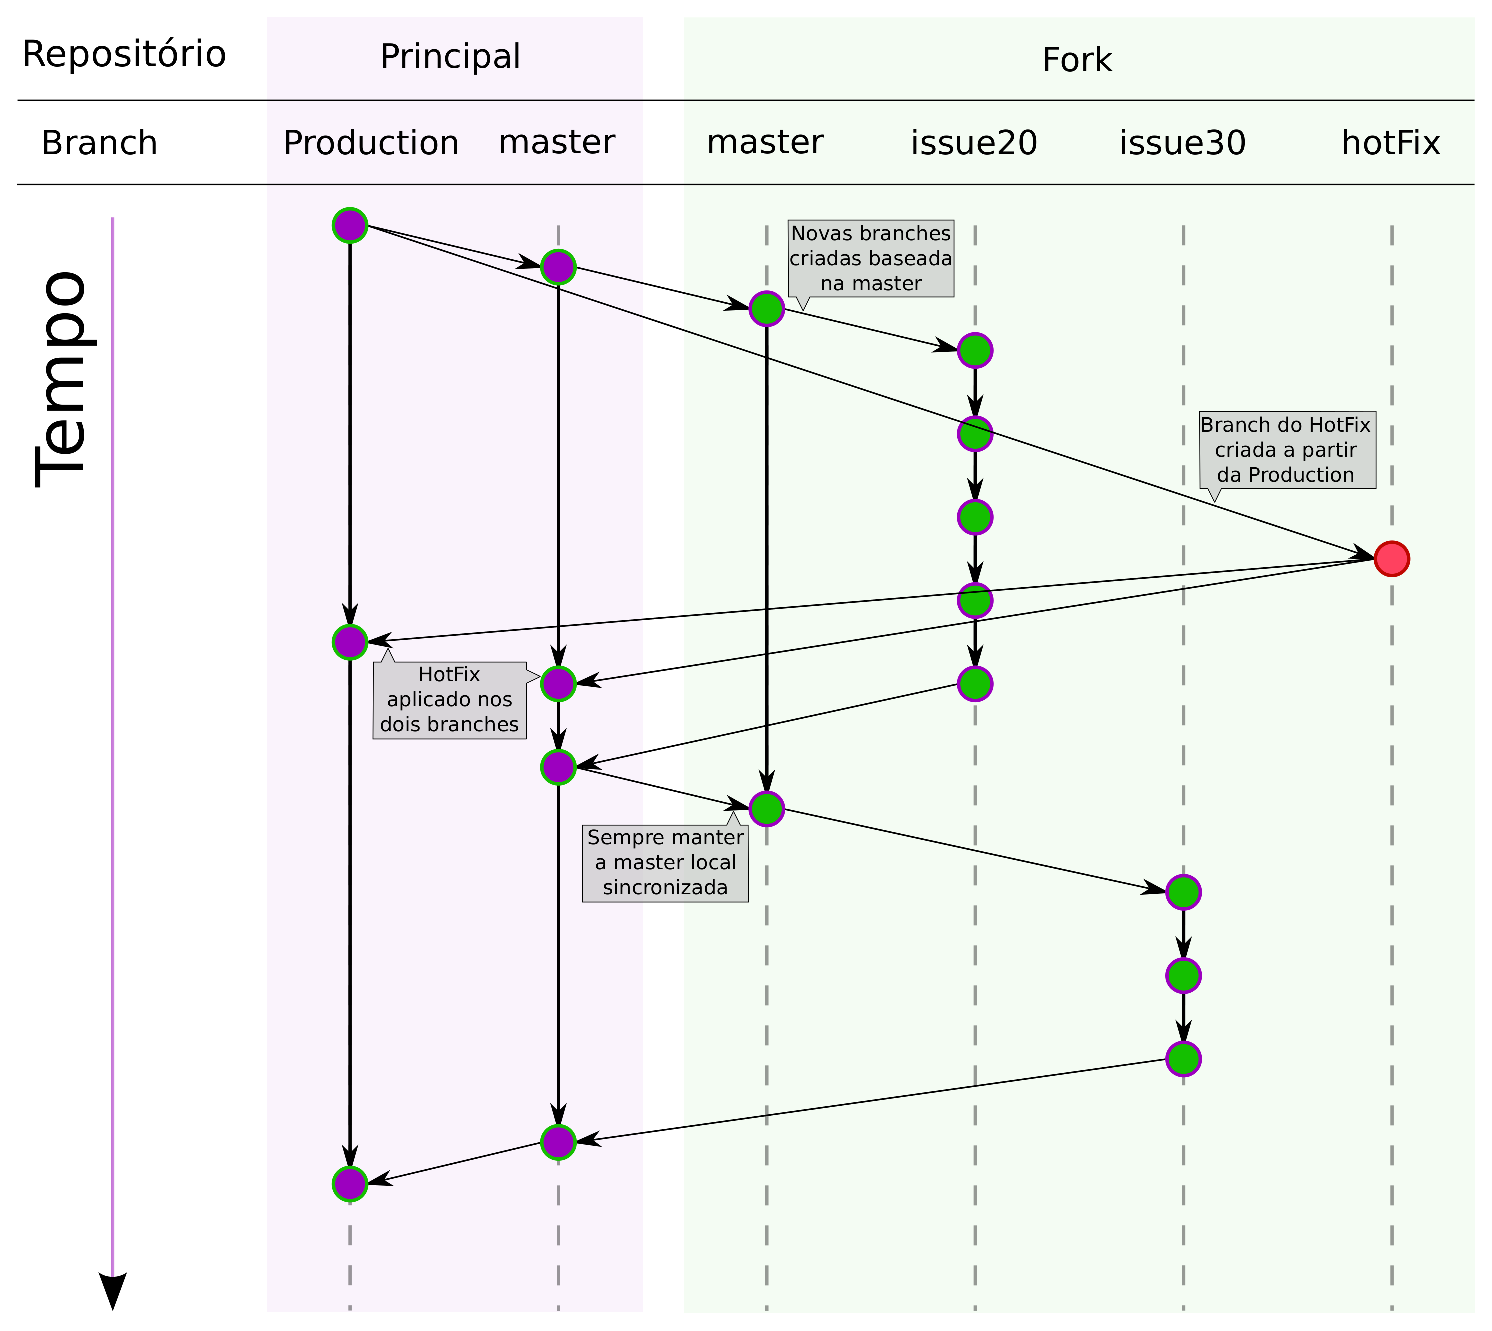
\includegraphics[scale=0.65]{./imagens/branchForkDiagram.eps}%
        \end{center}%
        \caption{Diagrama do Fluxo de Desenvolvimento \label{fig:gitflow}}%
        \fonte{Autoria Própria}%
    \end{figure}%
    
\clearpage
\subsection{Procedimento de integração de um \textit{Pull-Request}}
A integração de códigos desenvolvidos durante o \gls{sprint}, deve ser realizada no \gls{branch} \textbf{master} do projeto, para posteriormente ser transferida para o \gls{branch} \textbf{production}, que é o que estará em produção. É importante que o procedimento de integração não seja realizado utilizando a ferramenta de \gls{merge} da interface do GitHub, mas sim que seja realizado, de acordo com o que será apresentado abaixo, numa cópia local no computador da pessoal responsável pela integração.

O primeiro passo para integração de um \gls{pullrequest} é criar um novo \gls{branch} localmente, recomenda-se que o nome do \gls{branch} seja o nome da \gls{issue} a ser resolvida.
\begin{lstlisting}[language=bash,caption={Cria uma nova branch chamada issueXX baseada na branch master}]
git checkout -b issueXX master
\end{lstlisting}

O passo seguinte é incorporar as mudanças propostas no \gls{pullrequest}. As mudanças estão no repositório do(a) desenvolvedor(a) que originou o \gls{pullrequest}, na \gls{branch} de nome \textit{issueXX}.
\begin{lstlisting}[language=bash,caption={Recebendo as modificações do branch a ser incorporado}]
git pull https://github.com/<user>/<nome-do-repositorio>.git issueXX
\end{lstlisting}
Pode ser necessário realizar, manualmente, o trabalho de \gls{merge}, caso seja, é importante que a pessoa responsável pelo desenvolvimento do código que originou o \gls{pullrequest} esteja junto a quem está integrando os códigos para auxiliar na resolução do conflito.

Neste momento, o projeto local está com a modificação proposta implementada. Deve-se observar no \gls{pullrequest} que está no GitHub se existem observações relativas a mudanças que devem ser feitas no painel de administração do wordpress para completar a resolução da \gls{issue}. Caso existam, as recomendações devem ser seguidas e posteriormente registradas no wiki de documentação (\url{https://github.com/pensandoodireito/participacao-sitebase/wiki}) do projeto, na página relativa ao \gls{sprint} sendo avaliado.

Em seguida a equipe deve validar as modificações, verificando o resultado final. Caso decida-se que a \gls{issue} está resolvida, agora iremos integrar as mudanças na \gls{branch} \textbf{master} do projeto.
\begin{lstlisting}[language=bash,caption={Enviando as modificações aceitas para o branch master}]
git checkout master
git merge --no-ff issue37
git push origin master
\end{lstlisting}
